\tikzstyle{decision} = [diamond, draw, fill=blue!20, 
    text width=4.5em, text badly centered, node distance=3cm, inner sep=0pt]
\tikzstyle{block} = [rectangle, draw, fill=blue!20, text width=7em, text centered, minimum height=4em]
\tikzstyle{line} = [draw, -latex']
\tikzstyle{cloud} = [draw, ellipse,fill=red!20, node distance=3cm,
    minimum height=2em]
\tikzstyle{io} = [trapezium, trapezium left angle=70, trapezium right angle=110, draw, fill=blue!20,  text width=1em, text centered, minimum height=4em]

%\resizebox{!}{!}{%
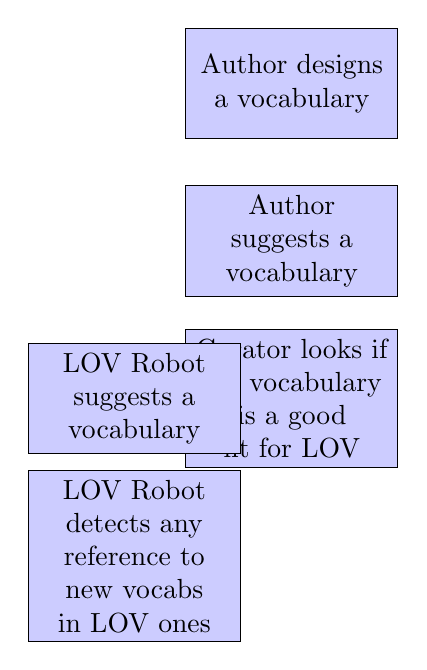
\begin{tikzpicture}[node distance = 2cm, auto]
    % Place nodes
%   \node [block] (init) {initialize model};
%    \node [cloud, left of=init] (expert) {expert};
%    \node [io, right of=init, xshift=2cm] (system) {system};
%    \node [block, below of=init] (identify) {identify candidate models};
%    \node [block, below of=identify] (evaluate) {evaluate candidate models};
%    \node [block, left of=evaluate, node distance=3cm] (update) {update model};
%    \node [decision, below of=evaluate] (decide) {is best candidate better?};
%    \node [block, below of=decide, node distance=3cm] (stop) {stop};
%    % Draw edges
%    \path [line] (init) -- (identify);
%    \path [line] (identify) -- (evaluate);
%    \path [line] (evaluate) -- (decide);
%    \path [line] (decide) -| node [near start] {yes} (update);
%    \path [line] (update) |- (identify);
%    \path [line] (decide) -- node {no}(stop);
%    \path [line,dashed] (expert) -- (init);
%    \path [line,dashed] (system) -- (init);
%    \path [line,dashed] (system) |- (evaluate);

% Place nodes
\node [block] (authDesigns) {Author designs a vocabulary};
\node [block, below of=authDesigns] (authSuggest) {Author suggests a vocabulary};
\node [block, below of=authSuggest] (curFit) {Curator looks if the vocabulary is a good fit for LOV};
\node [block, left of=curFit] (botSuggest) {LOV Robot suggests a vocabulary};
\node [block, below of=botSuggest] (botDetects) {LOV Robot detects any reference to new vocabs in LOV ones};
\end{tikzpicture}
%}